
\documentclass{Setup/template_isec_class}

% Template ISEC/LaTeX, janeiro 2023
%--------------------------------------
\usepackage{Setup/template_isec_package}
%--------------------------------------

%--------------------------------------
% Obs#1
% Onde incluir todos os ficheiros (package)
% e instruções adicionais para este projeto
\usepackage{extras}
%--------------------------------------

\begin{document}

%--------------------------------------
% Obs#2
% Definir qual o título e quais os autores do trabalho
\newcommand{\titulotrabalho}{Título do trabalho}
\newcommand{\autorestrabalho}{Autor ou autores do trabalho}
%--------------------------------------

\pagestyle{empty}

% Capa
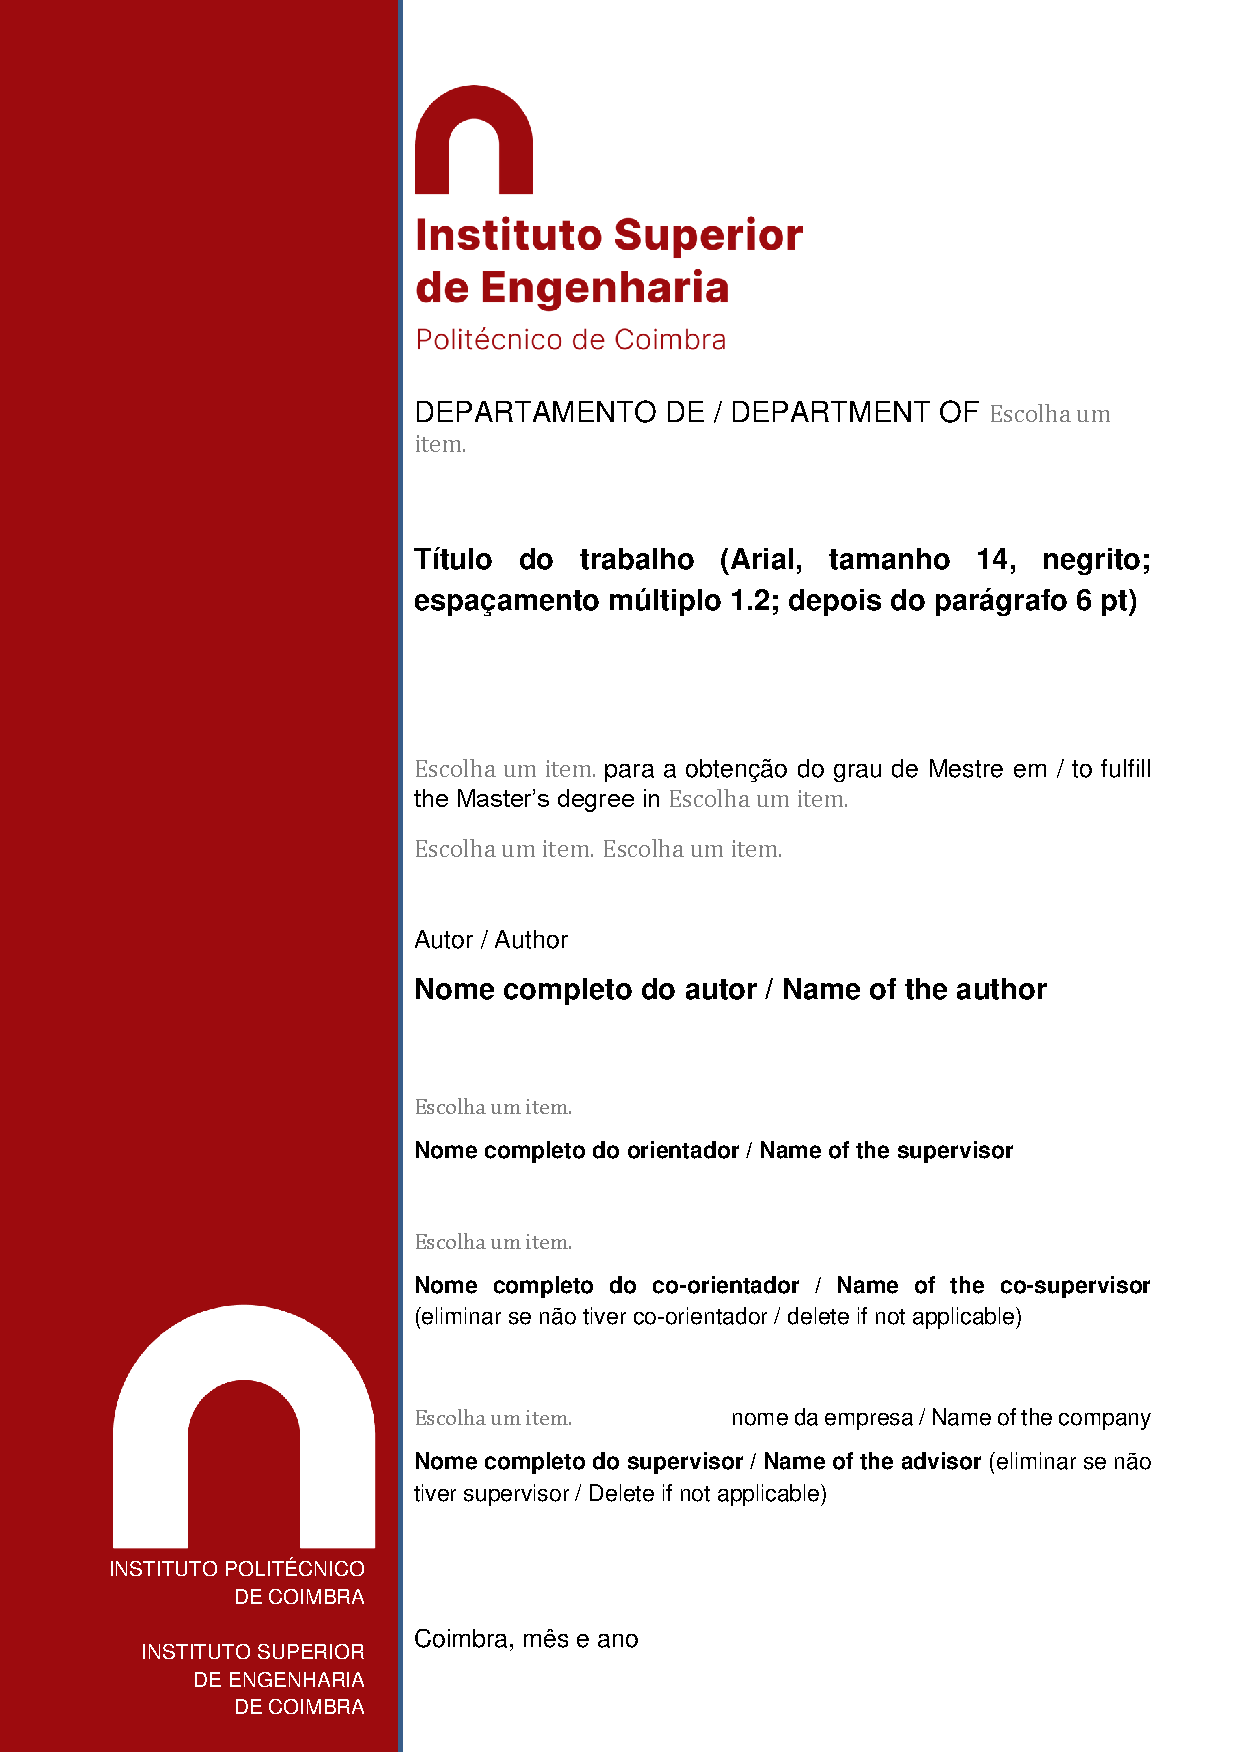
\includepdf{Inicio/capa}

\newpage

%--------------------------------------
\pagestyle{fancy}
\fancyhf{}
\fancyhead{}
\fancyhead[CO]{\nouppercase{\truncate{\headwidth}{\titulotrabalho}}}
\fancyhead[CE]{\nouppercase{\autorestrabalho}}
\renewcommand{\headrulewidth}{0pt}
\fancyfoot{}
\fancyfoot[CO,CE]{\thepage}
\setlength{\headheight}{14.5pt}
\fancypagestyle{plain}{}
%--------------------------------------

\pagenumbering{roman}

% Resumo PT
\phantomsection
\addcontentsline{toc}{chapter}{Resumo}

% Resumo
%--------------------------------------
\vspace*{45pt}
\begin{flushleft}
	{\Large \textbf{\scshape{Resumo}}}
\end{flushleft}
\vspace*{10pt}


\amostradetexto


\vspace*{20pt}

\noindent \textbf{Palavras-chave}:
palavra-chave1, palavra-chave2, palavra-chave3, palavra-chave4



\newpage

% Abstract ENG
\phantomsection
\addcontentsline{toc}{chapter}{Abstract}

% Abstract
%--------------------------------------
\vspace*{45pt}
\begin{flushleft}
	{\Large \textbf{\scshape{Abstract}}}
\end{flushleft}
\vspace*{10pt}


\amostradetexto


\vspace*{20pt}

\noindent \textbf{Keywords}:
keyword1, keyword2, keyword2, keyword3, keyword4



\newpage

% Epígrafe
\phantomsection
\addcontentsline{toc}{chapter}{Ep\'{\i}grafe}

% Epígrafe
%--------------------------------------
\vspace*{45pt}
\begin{flushleft}
	{\Large \textbf{\scshape{Ep\'{\i}grafe}}}
\end{flushleft}
\vspace*{10pt}

\begin{flushright}
	O começo de todas as ciências é o espanto de as coisas serem o que são. \\
	Aristóteles
\end{flushright}



\newpage

% Dedicatória
\phantomsection
\addcontentsline{toc}{chapter}{Dedicat\'{o}ria}

% Dedicatória
%--------------------------------------
\vspace*{45pt}
\begin{flushleft}
	{\Large \textbf{\scshape{Dedicat\'{o}ria}}}
\end{flushleft}
\vspace*{10pt}

Aqui poderá dedicar este trabalho a alguém que considere merecedor de tal distinção.


\newpage

% Agradecimentos
\phantomsection
\addcontentsline{toc}{chapter}{Agradecimentos}

% Agradecimentos
%--------------------------------------
\vspace*{45pt}
\begin{flushleft}
	{\Large \textbf{\scshape{Agradecimentos}}}
\end{flushleft}
\vspace*{10pt}


\amostradetexto



\newpage

\renewcommand{\contentsname}{\'{I}ndice}
\renewcommand{\listtablename}{\'{I}ndice de tabelas}
\renewcommand{\listfigurename}{\'{I}ndice de figuras}

\phantomsection
\addcontentsline{toc}{chapter}{\'{I}ndice}
\tableofcontents

\newpage

\phantomsection
\addcontentsline{toc}{chapter}{\'{I}ndice de tabelas}
\listoftables

\newpage

\phantomsection
\addcontentsline{toc}{chapter}{\'{I}ndice de figuras}
\listoffigures

\newpage

% Lista de abreviaturas
\phantomsection
\addcontentsline{toc}{chapter}{Lista de abreviaturas}

% Lista de abreviaturas
%--------------------------------------
\vspace*{45pt}
\begin{flushleft}
	{\Large \textbf{\scshape{Lista de abreviaturas}}}
\end{flushleft}
\vspace*{20pt}

\begin{tabular}{l l}
    IEEE	&  \textit{Institute of Electrical and Electronics Engineers}\\
    ISEC    &  Instituto Superior de Engenharia de Coimbra\\
    % deve acrescentar aqui as abreviaturas que considerar necessárias, por ordem alfabética    
\end{tabular}



\newpage

% Lista de símbolos
\phantomsection
\addcontentsline{toc}{chapter}{Lista de s\'{\i}mbolos}

% Lista de símbolos
%--------------------------------------
\vspace*{45pt}
\begin{flushleft}
	{\Large \textbf{\scshape{Lista de símbolos}}}
\end{flushleft}
\vspace*{20pt}

\begin{tabular}{l l}
    $\mathrm{kN}$       &   Quilonewton\\
    $\varepsilon_{ax}$  &   Extensão axial (\%)\\
    % deve acrescentar aqui os símbolos que considerar necessários, por ordem alfabética    
\end{tabular}



\newpage
\pagenumbering{arabic}

% Capítulo inicial
% Introdução

% Introdução
%--------------------------------------
\chapter{Introdução}


\amostradetexto



% Capítulo 2

% Segundo capítulo deste trabalho.
%--------------------------------------
\chapter{Exemplos de escrita em \LaTeX}
\label{cap2}

Neste capítulo são apresentados alguns exemplos que ajudam na elaboração e na organização de um documento escrito em \LaTeX. 

Na Secção \ref{cap2:sec_listas} são apresentados exemplos de listas com recurso aos comandos \textit{enumerate} e \textit{itemize}.  A utilização de símbolos em \LaTeX \ é exemplificada na Secção \ref{cap2:sec_simbolos}, onde está incluída uma nota de rodapé. Na Secção \ref{cap2:sec_def} são apresentadas definições, exemplos e proposições com o devido destaque. Equações e matrizes são descritas na Secção \ref{cap2:sec_equa}. Nas secções \ref{cap2:sec_tabelas} e \ref{cap2:sec_figuras} são apresentados exemplos de como definir uma tabela e de como incluir uma figura no documento, com a sua referência ao longo do texto. 

Fica a sugestão de apresentar uma pequena descrição do conteúdo de cada capítulo após a escrita do título do capítulo - como foi aqui ilustrado.

\section{Listas}\label{cap2:sec_listas}

    Segue um exemplo de um \textit{enumerate}:
    \begin{enumerate}
    	\item Primeiro item;
    	\item Segundo item;
    	\item Terceiro item.	
    \end{enumerate}
    
    Segue um exemplo de um \textit{itemize}:   
    \begin{itemize}
    	\item Primeiro item;
    	\item Segundo item;
    	\item Terceiro item.
    \end{itemize}
    
\section{Símbolos}\label{cap2:sec_simbolos}

    Alguns exemplos de símbolos gregos são $\Psi$, $\phi$, $\Theta$, $\theta$, $\mu$, $\rho$. Alguns símbolos matemáticos muitas vezes utilizados são os seguintes $\pi$, $\Rightarrow$, $\rightarrow$, $\infty$, $\geq$, $\neq$.

\subsection{Notas de rodapé}

    Para colocar uma nota de rodapé no texto basta colocar o respetivo texto dentro do comando \verb|\footnote|. Por exemplo\footnote{Exemplo de uma nota de rodapé.}.

\section{Etiquetas e respetiva referenciação no texto}

    Aquando da escrita de um documento é, por vezes, necessário referenciar um capítulo, uma secção, uma tabela, uma figura ou uma equação. Para o efeito deve-se utilizar o comando \verb|\label| junto ao elemento a referenciar e o comando \verb|\ref| para fazer a sua chamada no texto.

\section{Definições, exemplos e proposições}
    \label{cap2:sec_def}
    
    \begin{definition}
    Uma equação diferencial diz-se {\bf ordinária} se a
    função incógnita depende apenas de uma variável.
    \end{definition}
    
    \bigskip % para fazer um espaço na vertical
    
    \begin{example}
    São exemplos de equações diferenciais ordinárias as seguintes equações:
    \begin{enumerate}
    \item[(1)]
    $L\frac{d^2Q(t)}{dt^2}+R\frac{dQ(t)}{dt}+\frac{1}{C}Q(t)=E(t)$;
    \item[(2)] $L\frac{dI(t)}{dt}+RI(t)=E(t)$.
    \end{enumerate}
    \end{example}
    
   \bigskip
    
    \begin{proposition}
    Em qualquer triângulo retângulo, o quadrado do comprimento da hipotenusa é igual à soma dos quadrados dos comprimentos dos catetos.  
    \end{proposition}
    
\section{Equações e matrizes}
    \label{cap2:sec_equa}
    
    Nesta secção apresenta-se um exemplo de como definir uma equação numerada bem como a sua referenciação no texto.
    
    A velocidade em cada tecido $v_i,\, i=c,r,v$, pode ser definida por
    
    \begin{equation} 
        \label{Darcy_crv}
        \left\{
        \begin{array}{l}
            v_i=-\frac{k_i}{\mu_i}\nabla p_i \mbox{ in } \Omega_i\times (0,T],\\
            \nabla. v_i=0 \mbox{ in } \Omega_i\times (0,T], \quad i=c,r,v.
        \end{array}
        \right.
    \end{equation}
    
    Na Equação (\ref{Darcy_crv}), $k_i$ representa a permeabilidade do tecido e $\mu_i$ representa a viscosidade do fluido. 
    
    Um exemplo de uma equação centrada no texto sem numeração apresenta-se de seguida.
    
    $$ \gamma_r=\left\{
        \begin{array}{l}
            \gamma_{r,1}  \mbox{ in } \Omega_{r,1},\\
            \gamma_{r,2}  \mbox{ in } \Omega_{r,2}.
        \end{array}
        \right. $$
    
    Um exemplo de uma matriz quadrada é
        \begin{equation}
        M_{3,3}=\left[ \begin{array}{ccc}
                  1&2&3\\
                  4&5&6\\
                  7&8&9
                \end{array}
            \right].\label{matriz}
        \end{equation}     
    A Matriz (\ref{matriz}) tem ordem três. Pode-se  definir uma matriz arbitrariamente grande como, por exemplo, a matriz tridiagonal que se segue:
    
    $$A=\frac{1}{\Delta x^2}\left[ 
        \begin{array}{ccccccc}
               -2\alpha & \alpha-\frac{\beta\Delta x}{2} & 0 & 0 & \cdots & 0 & 0 \\
               \alpha-\frac{\beta\Delta x}{2} & -2\alpha & \alpha+\frac{\beta\Delta x}{2} & 0 & \cdots & 0 & 0 \\
               0 & \alpha-\frac{\beta\Delta x}{2} & -2\alpha & \alpha+\frac{\beta\Delta x}{2} & \cdots & 0 & 0 \\
               \vdots & \vdots & \vdots  & \vdots & \ddots & \ddots & \vdots \\
               0 & 0 & 0 & 0& \cdots& -2\alpha & \alpha+\frac{\beta\Delta x}{2} \\
               0 & 0 & 0 & 0& \cdots& 0 & -2\alpha 
        \end{array}
    \right].$$
    
\section{Tabelas}
    \label{cap2:sec_tabelas}
    
    Segue-se um exemplo de uma tabela em que o conteúdo da primeira coluna está alinhado à esquerda e em que o conteúdo das restantes colunas está centrado, Tabela~\ref{tab_sem_separadores}.  Cada tabela deve ter um título/legenda,  sendo possível associar-lhe uma referência para ser identificada ao longo do texto.
    
    \begin{table}[htp]
    \caption{\small Um exemplo de uma tabela.}
    \label{tab_sem_separadores}
    \centering
    	\begin{tabular}{l|ccc} \hlinewd{2pt}
    		Comparação   & Vítreo & Retina & Coróide \\ 
                \hline
    		SCS com Iont. \textit{vs} No Iont. &  20\% & 7\%&1\% \\
    		SRS com Iont. \textit{vs} No Iont. & 45\% & 14\%&8\% \\
    		SCS com Iont. \textit{vs} Intravitreal &-80\% & 150\% & 2000\% \\
    		SRS com Iont. \textit{vs} Intravitreal & -90\% & 1002\% & 2300\% \\  
    		\hlinewd{2pt}
    	\end{tabular}
    \end{table}
    
    Um exemplo de tabela com separadores entre colunas e todas as celulas centradas apresenta-se na Tabela~\ref{tab_com_separadores}.
    
    \begin{table}[htp]
    \caption{\small Outro exemplo de uma tabela.} 
    \label{tab_com_separadores}
    \centering
    		\begin{tabular}{c|c|c} 
                    \hlinewd{2pt}
    			Tipo de administração & Concentração máxima & Instante \\        \hline
    			SCS com Iont & 0.0034 & 19.7  \\
    			SRS com Iont & 0.0034 & 32  \\
    			Injeção IVI  & 0.0055 & 36.7 \\
    			\hlinewd{2pt}
    		\end{tabular}
    \end{table}
    
    No endereço \verb|https://www.tablesgenerator.com/| poderá encontrar uma forma automatizada de gerar tabelas em \LaTeX.
   
\section{Figuras}
\label{cap2:sec_figuras}

    Para inserir uma figura no texto (em formato PNG) pode ser utilizado o comando \verb|\includegraphics|. É também possível definir com este comando uma etiqueta que permite referenciar a figura no texto, assim como fornecer a legenda da figura.

    \begin{figure}[htp]
    	\centering	
            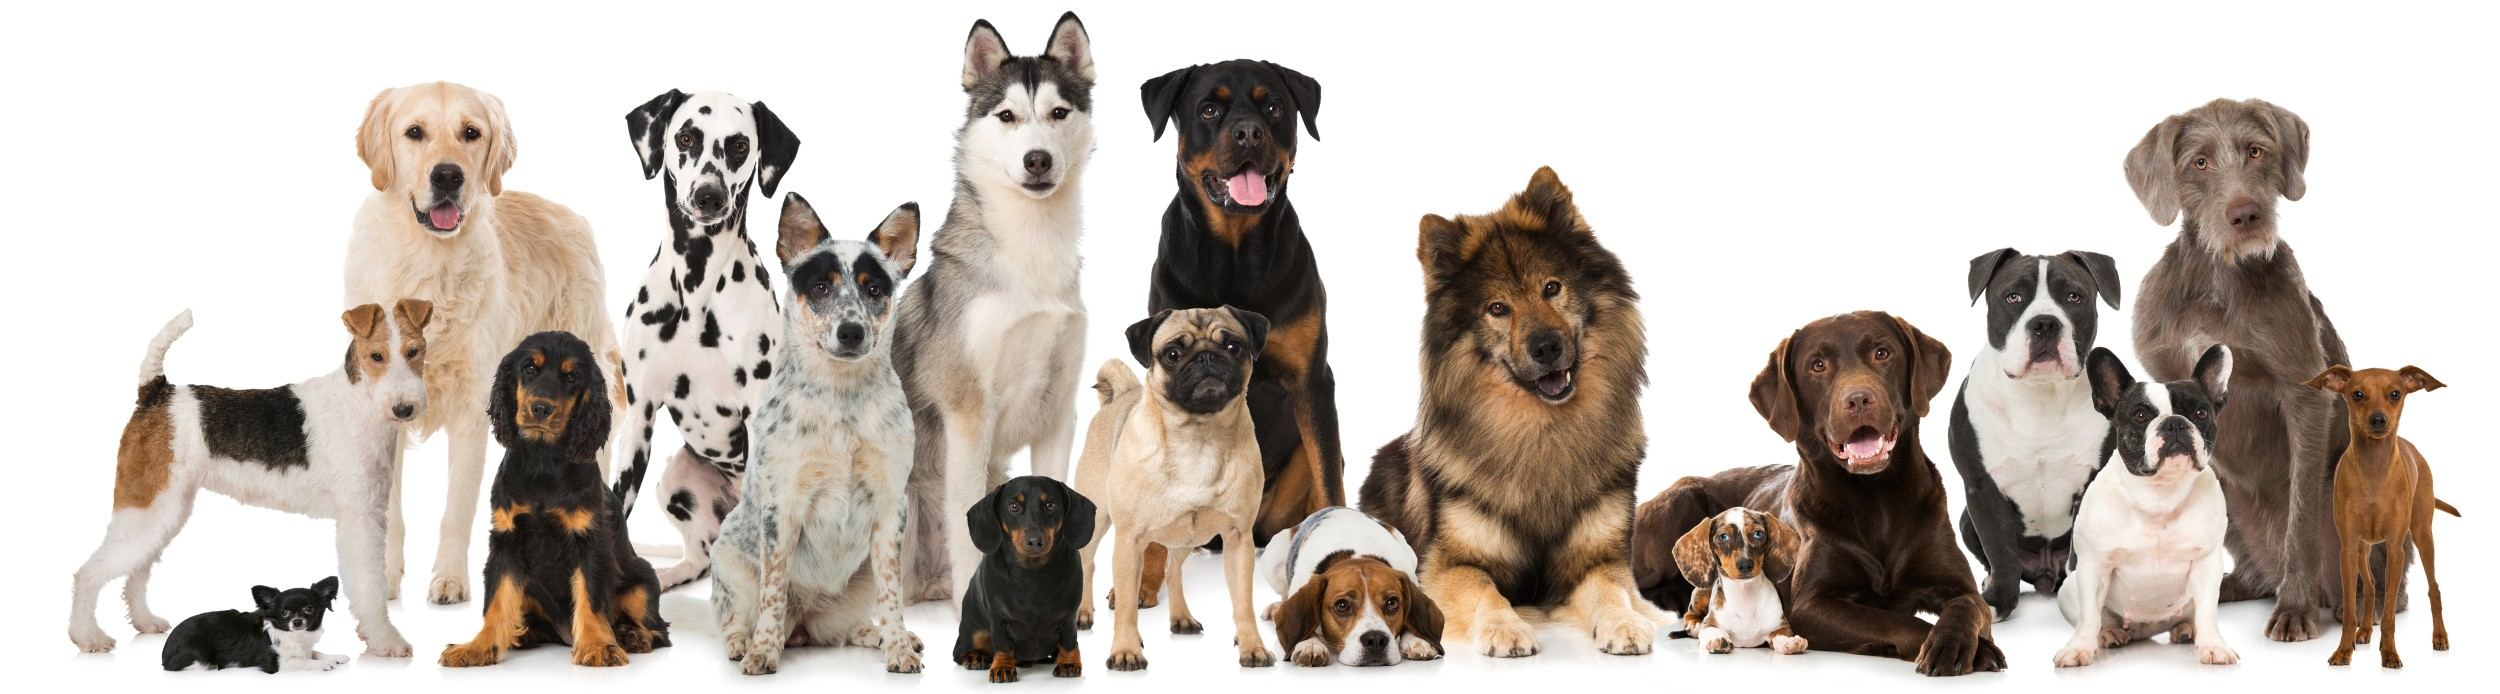
\includegraphics[width=0.8\textwidth]{Figuras/caes}
            \caption{\small Algumas raças caninas \cite{CitekeyPhdthesis}.}
    	\label{fig_caes_sem_foot}
    \end{figure}
    
    \begin{figure}[htp]
    	\centering
    	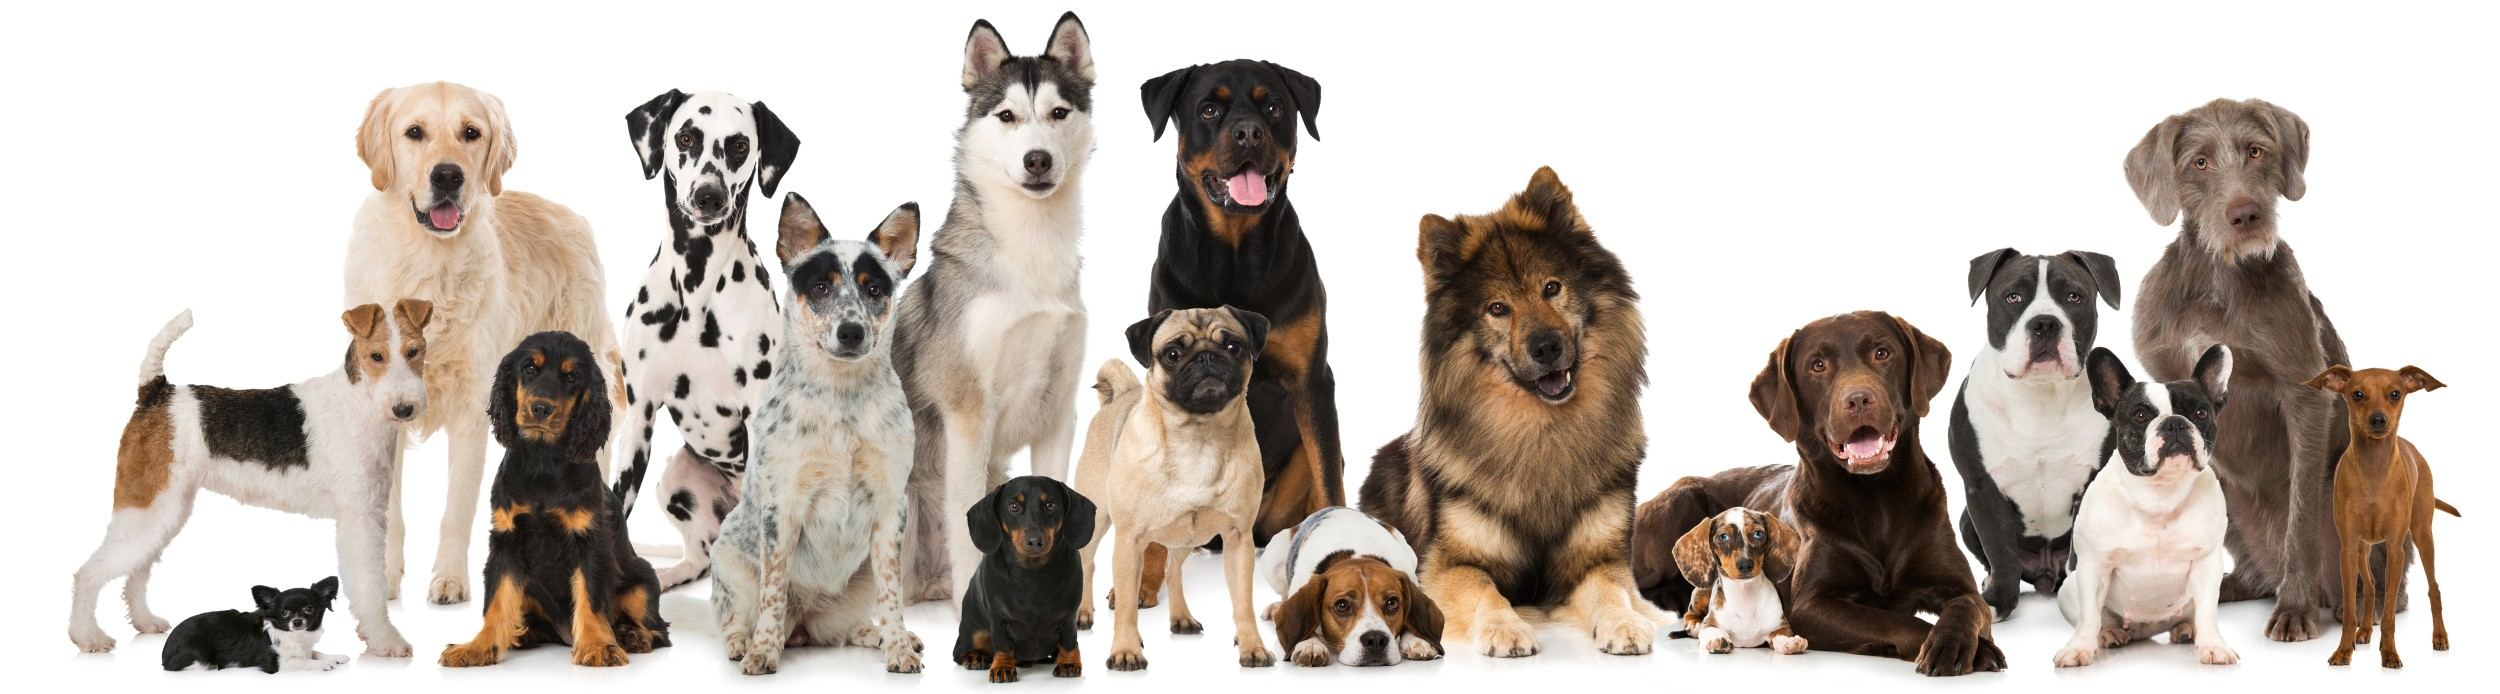
\includegraphics[width=8cm]{Figuras/caes}
            \caption[\small Algumas raças caninas com outro tamanho.]{\small Algumas raças caninas com outro tamanho\footnotemark.}
    	\label{fig_caes_com_foot}
    \end{figure}

    \begin{figure}[htp]
         \centering
         \begin{subfigure}[b]{0.3\textwidth}
             \centering
             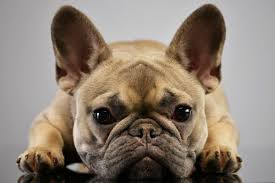
\includegraphics[width=\textwidth]{Figuras/buldog}
             \caption{}
             \label{fig:a}
         \end{subfigure}
         \hfill
         \begin{subfigure}[b]{0.3\textwidth}
             \centering
             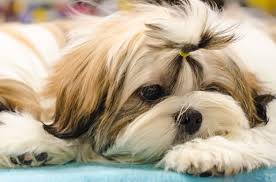
\includegraphics[width=\textwidth]{Figuras/shih_tzu}
             \caption{}
             \label{fig:b}
         \end{subfigure}
         \hfill
         \begin{subfigure}[b]{0.3\textwidth}
             \centering
             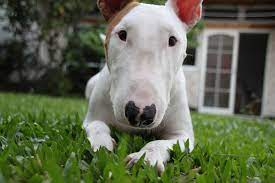
\includegraphics[width=\textwidth]{Figuras/bull_terrier}
             \caption{}
             \label{fig:c}
         \end{subfigure}
            \caption{\small Três raças de cães. (a) Bulldog; (b) Shih Tzu; (c) Bull Terrier.}
            \label{fig_c}
    \end{figure}
    
    Na Figura~\ref{fig_caes_sem_foot} são ilustradas algumas raças caninas. Na Figura~\ref{fig_caes_com_foot} é apresentada a figura anterior com a inclusão de uma nota de rodapé. As duas figuras apresentam duas formatações possíveis para o tamanho da figura. Na Figura~\ref{fig_caes_sem_foot}, o tamanho da imagem é definido relativamente à largura do texto (neste caso corresponde a 80\% da largura do texto). Já na Figura~\ref{fig_caes_com_foot}, a figura tem a largura absoluta de $8~cm$.   
    Um exemplo onde são colocadas três imagens lado a lado, indicando a referência de cada uma das imagens recorrendo a um só  \textit{label}, está apresentado na Figura~\ref{fig_c}. Na Figura~\ref{fig:b} pode visualizar-se um cão da raça Shih Tzu.
    
    \footnotetext{Fonte: \textit{https://images.app.goo.gl/HhdCXAy6DVtBYjsF9}}
    
    

% Capítulo 3

% Terceiro capítulo deste trabalho.
%--------------------------------------
\chapter{Citações e estilos de referências}
\label{cap3}

Este é o terceiro capítulo deste trabalho. 
Na Secção \ref{cap3:citacoes} é indicado como citar uma referência bibliográfica. Os estilos a adotar para as referências bibliográficas são descritos na Secção \ref{cap3:estilosRef}.

\section{Citações}
\label{cap3:citacoes}
    
    Para citar no texto um trabalho previamente incluído nas referências bibliográficas, deve apenas usar-se o comando \verb|\cite| e o respetivo identificador associado a cada uma das referências. 
    
    \subsection{Alguns exemplos}
    
    Aqui pode encontrar exemplos de citações de um artigo \cite{Cohen:1963}, de um livro \cite{CitekeyBook}, de uma secção de um livro \cite{CitekeyInbook}, de um artigo publicado nas atas de um evento \cite{CitekeyInproceedings}, de uns \textit{proceedings} \cite{CitekeyProceedings}, de um manual \cite{CitekeyManual}, de uma tese de mestrado \cite{CitekeyMastersthesis}, de uma tese de doutoramento \cite{CitekeyPhdthesis}, de um relatório técnico \cite{CitekeyTechreport}  
    e de uma referência que não se insere nas categorias anteriores \cite{CitekeyMisc}.
    Se for necessário citar mais do que um trabalho no mesmo ponto do texto, basta separar os trabalhos por vírgulas dentro do comando \verb|\cite|. A título de exemplo, podem citar-se três trabalhos em simultâneo da seguinte forma \cite{Cohen:1963, CitekeyBook,CitekeyInbook}.

\section{Estilo a adotar para as referências bibliográficas}
    \label{cap3:estilosRef}
    
    Os alunos podem escolher utilizar o estilo IEEE ou o estilo APA.
    
    \subsection{Estilo APA}
    \label{cap3:estiloAPA}
    
    Para escolher o estilo APA, deve aceder ao ficheiro \verb+extras.sty+ e procurar por Obs\#1 e descomentar a linha relativa à instrução \verb+\usepackage{apacite}+. \\
    Adicionalmente, no ficheiro \verb+main.tex+ deve procurar a Obs\#3 e descomentar a instrução \verb+\bibliographystyle{apacite}+ e comentar \verb+\bibliographystyle{IEEEtran}+.
    
    \subsection{Estilo IEEE}
    Para escolher o estilo IEEE, deve fazer o procedimento inverso ao descrito na Subsecção \ref{cap3:estiloAPA}, ou seja, deve comentar a instrução \verb+\usepackage{apacite}+ no ficheiro \verb+extras.sty+ (procurar por Obs\#1) bem como comentar a linha \verb+\bibliographystyle{apacite}+ e descomentar a linha \verb+\bibliographystyle{IEEEtran}+ no ficheiro \verb+main.tex+ (procurar por Obs\#3). 
    
    
    

% Capítulo final
% Conclusão

% Conclusão
%--------------------------------------
\chapter{Conclusão}


\amostradetexto



\newpage

% Referências bibliográficas
\phantomsection
\addcontentsline{toc}{chapter}{Refer\^{e}ncias bibliogr\'{a}ficas}
\renewcommand{\bibname}{Refer\^{e}ncias bibliogr\'{a}ficas}

%-------------------
% Obs#3
% Descomentar uma das seguintes linhas, em alternativa, 
% consoante o estilo pretendido para as referências bibliográficas
\bibliographystyle{IEEEtran} % formatação segundo IEEE 
%\bibliographystyle{apacite} % formatação segundo APA 
%-------------------
\bibliography{bibliografia}

\newpage

% Anexos
\phantomsection
\addcontentsline{toc}{chapter}{Anexos}
\chapter*{Anexos}

\newpage

% Anexo A
%--------------------------------------
% Obs#4
% Definir o título do anexo A
\newcommand{\tituloanexoA}{Título do Anexo A}
%--------------------------------------
\phantomsection
\addcontentsline{toc}{section}{Anexo A - \tituloanexoA}

% Anexo
%--------------------------------------
\vspace*{45pt}
% Título do anexo A (\tituloanexoA) definido no ficheiro main
\section*{Anexo A - \tituloanexoA}


%tira a próxima linha e escrever o anexo A
\amostradetexto


\newpage

% Anexo B
%--------------------------------------
% Obs#5
% Definir o título do anexo B
\newcommand{\tituloanexoB}{Título do Anexo B}
%--------------------------------------
\phantomsection
\addcontentsline{toc}{section}{Anexo B - \tituloanexoB}

% Anexo
%--------------------------------------
\vspace*{45pt}
% Título do anexo B (\tituloanexoB) definido no ficheiro main
\section*{Anexo B - \tituloanexoB}


%tira a próxima linha e escrever o Anexo B
\amostradetexto



\newpage

\thispagestyle{empty}

% Última página

% Última página
%--------------------------------------

\pagecolor{IsecVermelho}

\mbox{}

\vfill

\begin{center}

\includegraphics[scale=0.3]{Setup/isec-logo}
\end{center}

\newpage

\pagecolor{white}



\end{document}

